\documentclass{article}
\usepackage[utf8]{inputenc}
\usepackage{graphicx}
\usepackage{amsmath}
\usepackage{hyperref}
\usepackage[a4paper, textwidth=450pt]{geometry}

\graphicspath{ {./data/} }

\title{E17e Coupled Electrical Oscillations Report}
\author{Adam Kit}
\date{May 2020}


\begin{document}

\maketitle

\section*{Preperation}
In this experiment two \textit{LC} resonant circuits are coupled either by a capacitance or by a mutual inductance. The capacitor in one of the circuits is charged by applying a DC voltage. This circuit is excited to oscillations by the subsequent removal of the voltage and the coupled oscillations of both circuits aremeasured as a function of time. From this the resonant frequencies are determined and their dependence on coupling capacitance or mutual inductance is studied.

To set this up, Prof. Ziesse provided us with data recorded using a PC Oscilloscope. Instead of using Origin, I chose to work using python, utelizing the pandas, numpy, and scipy libraries. I justify my choice by the fact that I will have to greatly depend on these libraries if I am to work in the simulation field of study, so I must begin now my preperation. All graphs are then made with matplotlib, and the github repository for each Lab can be found \href{https://github.com/fusionby2030/Numerical_Methods/tree/master/Labs/E17e}{here}.
\subsection{Fourier  Coefficients}
To approximate a function with a Fourier series we need a periodic bounded function that is integrable over a period $T$. If that is achieved, then we can write the function as the following series:
\begin{equation}
f(x) = a_0 + \sum_{n=1}^{\infty}[a_n cos(\omega_n t)+ b_nsin(\omega_n t)]
\end{equation}
where frequency $\omega_n$ is defined by $\omega_n = \frac{2 \pi n}{T}$. The coefficients are then found with the following equations
\begin{equation}
a_0 = \int_0^T f(t)dt
\end{equation}
\begin{equation}
a_n = \frac{2}{T}\int_{-\frac{T}{2}}^{\frac{T}{2}} f(t)cos(\omega_nt)dt
  \quad\text{and}\quad
b_n = \frac{2}{T}\int_{-\frac{T}{2}}^{\frac{T}{2}} f(t)sin(\omega_nt)dt
\end{equation}
\\ \\ \\
For the square wave represented in Figure \ref{swave} we use 1, 2, and 3 to find the first 6 coefficients of the fourier series if $T = 2\pi$ and $\omega_n = \frac{2 \pi n}{T} = n$

\begin{figure}[h]

  \centering
  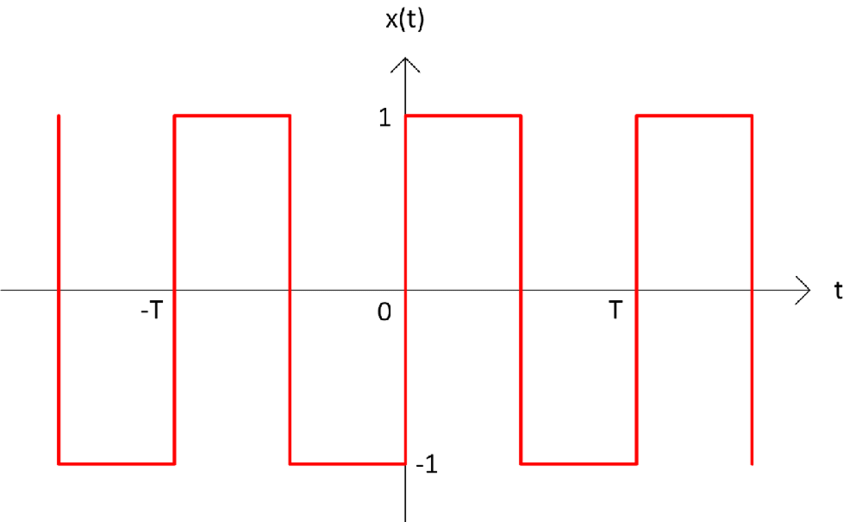
\includegraphics[scale=0.3]{squarewave.png}
  \caption{A simple square wave. These can be defined by $x(t) = sgn(sin(\frac{\omega t}))$ where $sgn(t)$ is the sign function that is $1$ if $ t > 0$, $0$ if $ t = 0$ and $-1$ if $ t < 0$}
  \label{swave}

\end{figure}

$$a_0 = \int_0^T f(t)(dt) = 0$$
$$a_1 = \frac{1}{\pi} \int_{-\pi}^{\pi} f(t)cos(t) = 0$$
$$a_2 = \frac{1}{\pi} \int_{-\pi}^{\pi} f(t)cos(2t) = 0 $$
and since the integral of $cos(t)$ from the intervals $-\pi$ to $\pi$ is always 0, we can say $a_n = 0$. As for the sin part of the fourier series: \\
$$b_1 = \frac{1}{\pi} \int_{-\pi}^{\pi}f(t)sin(t) = \frac{-1}{\pi}\int_{-\pi}^{0} sin(t)dt + \frac{1}{\pi}\int_0^{\pi} sint(t)dt= \frac{-1}{\pi}(-2) + \frac{1}{\pi} (2) = \frac{4}{\pi}$$
$$b_2 = \frac{-1}{\pi} \int_{-\pi}^{0}sin(2t)dt + \frac{1}{\pi}\int_{0}^{\pi}sin(2t)dt = 0 $$
$$b_3 = \frac{-1}{\pi}\int_{-\pi}^{0}sin(3t)dt + \frac{1}{\pi}\int_{0}^{\pi}sin(3t)dt = \frac{-1}{\pi}(\frac{-2}{3}) + \frac{1}{\pi}(\frac{2}{3})= \frac{4}{3\pi} = \frac{b_1}{3}$$
concluding that $b_n = \frac{4}{n\pi}$ when $n$ is odd, but $0$ otherwise. This greatly simplifies our Fourier Series, reducing it only to a series of sin waves! This is meaning that the function is odd.
\begin{equation}
f(t) = \frac{4}{\pi}\sum_{n=1}^{\infty} \frac{sin(\omega(2k-1)t)}{2k-1}
\label{squarefunction}
\end{equation}
Thus we can approximate the square wave using with 6 coefficients $(n = 6)$ as the following: \\ \\ $$f(t) = \frac{4}{\pi}[sin(t) + \frac{sin(3t)}{3} + \frac{sin(5t)}{5}] $$
One can see this done in the github repository for this lab. The file for graphing is : INSERT GITHUB HERE  \\ \\

For the Triangle wave, we start with deriving the fourier coefficients just like for the square wave. With $2L = T$,  The function $f(t)$ within the range $\frac{-T}{2} \leq t \leq \frac{T}{2}$ is given by: \\
\[
f(t) =
  \begin{cases}
    \text{$\frac{2t}{T}$} &\quad\text{: 0}\le\text{t}\le\text{T/2}\\
    \text{$-\frac{2t}{T}$} &\quad\text{: T/2}\le\text{t}\le\text{T} \\
  \end{cases}
\]
then the coefficients for b are given by (since just like the square wave, the triangle wave is also odd) \\ \\
\begin{equation}
b_n = \frac{2}{L} \{\int_0^{L/2}\frac{t}{L/2}sin(\frac{n\pi t}{L})dt + \int_{L/2}^{L}[2-\frac{2t}{L}]sin(\frac{n\pi t}{L})dt \} = \frac{32}{\pi^2 n^2} cos( \frac{1}{4} n \pi ) sin^3(\frac{1}{4}n\pi)
\label{triwavecoef}
\end{equation}

Here we denote the relationship between $n$ and $cos( \frac{1}{4} n \pi ) sin^2(\frac{1}{4}n\pi)$.

\[
cos( \frac{1}{4} n \pi ) sin^2(\frac{1}{4}n\pi) =
  \begin{cases}
    \text{0} &\quad\text{n = 0,4,8, ...} \\
    \text{$\frac{1}{4}$} &\quad\text{n = 1,5,9, ...} \\
    \text{0} &\quad\text{n = 2,6,10, ...} \\
    \text{$-\frac{1}{4}$} &\quad\text{n = 3,7,11 ...} \\
  \end{cases}
\]
Thus dividing the constant infront in equation \ref{triwavecoef}, we have the relationship:
\[
\frac{8}{\pi^2 n^2}
  \begin{cases}
    \text{0} &\quad\text{n = 2,6,10, ...} \\
    \text{$(-1)^{(n-1)/2}$} &\quad\text{n = 3,7,11 ...}
  \end{cases}
\]
And the Fourier Series is then
\begin{equation}
f(t) = \frac{8}{\pi^2} \sum_{n=1,3,5,...}^{\infty} \frac{(-1)^{(n-1)/2}}{n^2}sin(\frac{n\pi t}{L}) = \frac{8}{\pi^2} \sum_{i=0}^{N-1}(-1)^in^{-2}sin(2\pi f nt)
\label{trianglewaveeq}
\end{equation}
The last equation, we subsituted $n$ for the harmonic label $i$ where $n = 2i+1$ and period $L$ for frequency $f$ where $1/L = 2f$.



\subsection{FFT}
In Figure \ref{allWaveFFT} we see the waves and their respective FFT. The sin wave has a phase difference of $\pi /3$. The bottom row represents the signals in the frequency domain using the FFT function. The FFT computes N-point complex DFT, which we must then take the absolute value of to get the amplitude spectrum.
\begin{figure}[h]
  \centering
  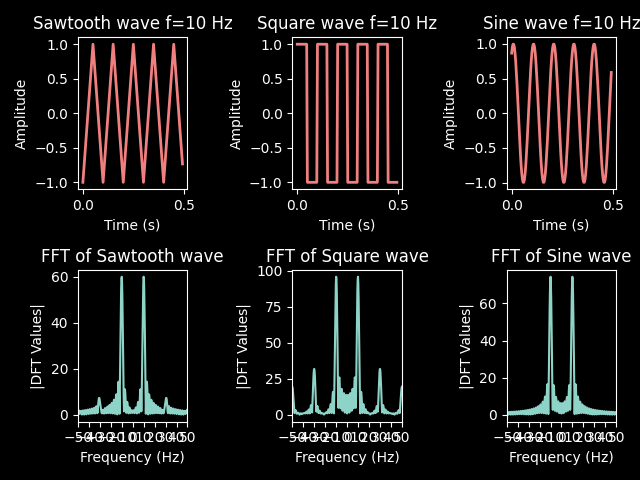
\includegraphics[scale=0.6]{allFTT.png}
  \caption{The comparison of a waves and their FFT}
  \label{allWaveFFT}
\end{figure}

\subsection{Comparison}
We compare in Figure \ref{sinvscos} the Phase Spectrums (left) and FFT Amplitude Spectrums (right). The frequency $f$ for both waves is $44.5$kHz. The FFT Spectrums show us where the signal lies within each given frequency, and this is sometimes much more usefull than trying to make sense of things in the time domain. In the Phase Spectrums, we graph $tan^{-1}(\frac{A_{im}}{A_{real}})$ where A represents the amplitude values for each respective wave. Then, filtering out values below the max, we see that the maximum values are occuring at the phases

\begin{figure}[h]
  \centering
  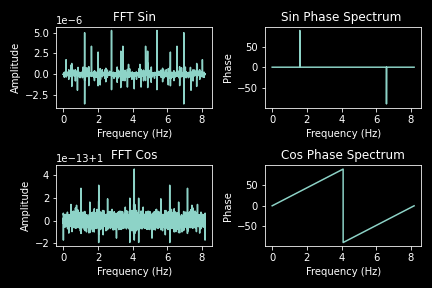
\includegraphics[scale=0.6]{sinvscos.png}
  \caption{The comparison of the Phase and Amplitude Spectrums of Sin and Cos signals generated by their FFT}
  \label{sinvscos}
\end{figure}

And lastly we compare the spectra of the function $sin(2\pi f_1 t)cos(2\pi f_2 t)$. In the Figure \ref{freqsine} we see two cases on the top row, where the left has frequecies $f_1= f_2$ and the right has $f_1 = 10f_2$, where $f_2 = 2Hz$ (beat frequency). On the bottom row we see the comparison between $sin(2\pi f_1 t)cos(2\pi f_2 t)$ (left) and $cos(2\pi f_1 t)sin(2\pi f_2 t)$.

\begin{figure}[h]
  \centering
  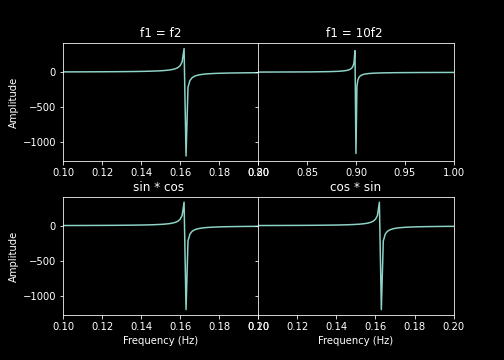
\includegraphics[scale=0.6]{freqsin.png}
  \caption{The comparison of how frequency affects certain signals FFT}
  \label{freqsine}
\end{figure}
The change in frequency across the top row leads to slight shifts in the corresponding spectrums, as is expected when you shift frequencies.  As for the bottom row, we notice there is no difference when you multipy first the sin vs the cos. I suppose there is not much of a change because one is not really changing much about the equation, and when multiplying and adding waves together, we know that the resultant frequency is a combination of the two resonant frequency, thus since these are not changing when you structure the order of multiplication, the final frequency will not change.
\section{Task 1}
\subsection{Aliasing}
Explain what the alias effect is. Why do these measurements prove the alias effect? If a measurement is made of a sine voltage with a frequency of 44.5 kHz with oscilloscope settings as shown to the right, how does the spectrum look like?
\begin{figure}[h]
  \centering
  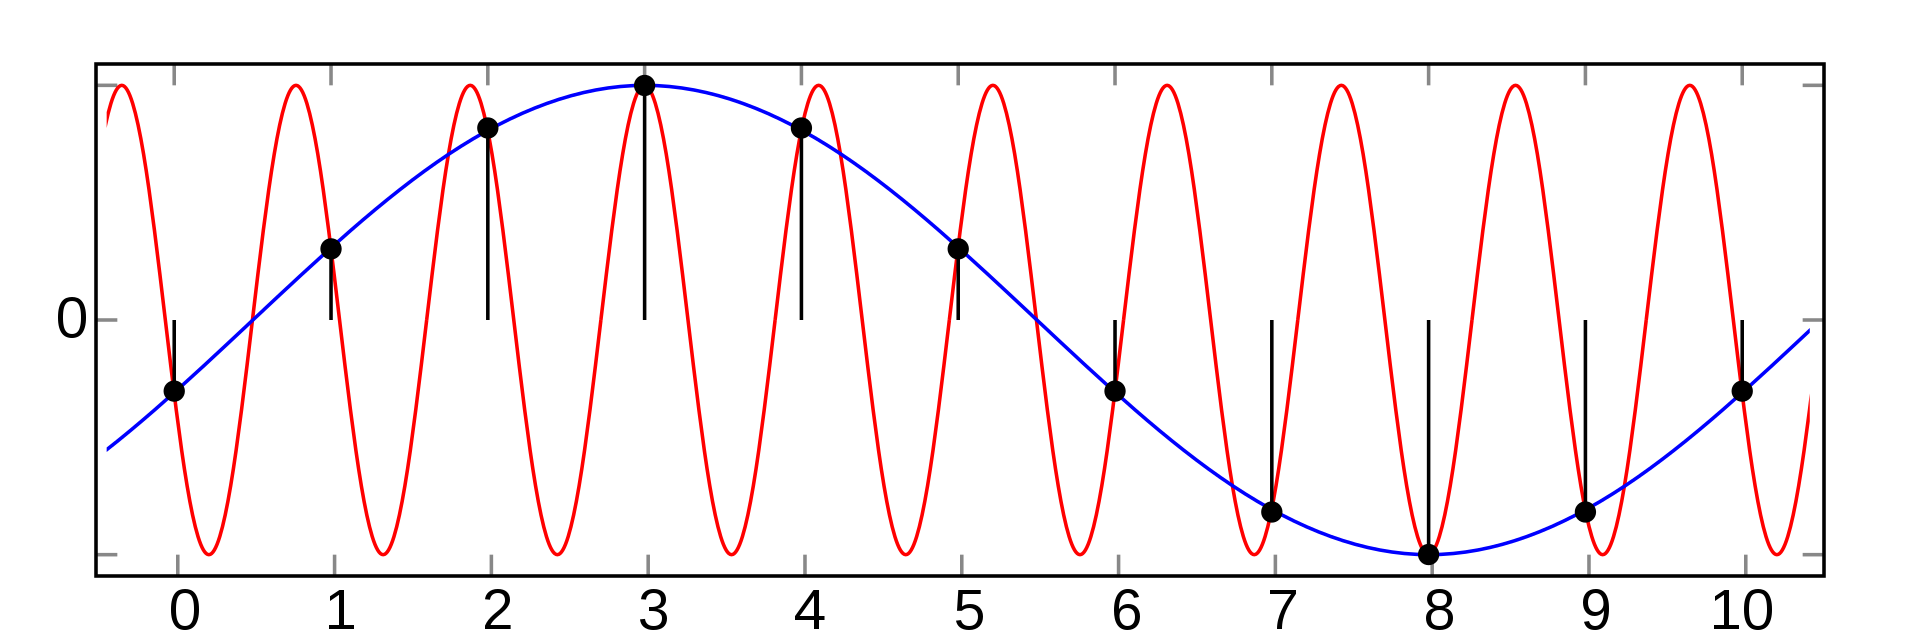
\includegraphics[scale=0.09]{aliassine.png}
  \caption[scale=0.5]{Two different sinusoids that fit the same set of samples.}
  \label{aliassine}
\end{figure}
Aliasing matters when one attempts to reconstruct the original waveform from its samples.
In Figure \ref{aliassine} a plot depics a set of samples with sample frequency $f_s =1$, but the red wave goes through 9 cycles while the blue only 1 on the span of 10 samples. So these two different signals become virtually indistinguishable when sampled!

For the two images given in the Lab Explanation, we see two completely different signals transformed into the Frequency domain to produce spectrums that are nearly identical. Although they both have the same sampling rate and number of samples, they are still able to produce similar Spectrums. This is not so strange, as sinusoids can be modeled by a combination of many sinusoids of different frequences (See Preperation on Fourier Coef.) So given that both signals are sine waves, even though they operate at different frequencies, it is entirely likely that one signal can decompose into the other, and vice versa.
\\
\subsection{Square Voltage}
Why do the spectra look so different? Compare qualitatively to your calculations from task 0.
\\
The frequencies differ by a magnitude of $0.1$ kHz, which I thought would not lead to such differences in spectra, as the square wave is really just a sum of many sine waves, however since $\omega = 2\pi f$, we see that if $f$ is any odd integer multiple, then for every sin in \ref{squarefunction} will tend to one when integrated! Thus the slight change in frequency, 1 to 1.1, will lead to a very big change in the overall spectrum graph.


\subsection{Triangular Voltage}
Why do the spectra look so different? Compare qualitatively to your calculations from task 0.Why does the lower time trace consist of a triangular pattern? \\
Once again the frequencies vary by 0.1kHz, so when we are using \ref{trianglewaveeq} we see also something similar. Again with $\omega = 2\pi f$ we will have a sin function that when the FFT comes for it during its Fourier Transformation, will turn into a one if $f$ is some odd integer multiple. Thus a slight change to 1.1kHz is bound to cause great disruption in the frequency spectrum of a Triangle signal.
\section{Task 2}
\subsection{Pre-Experiment}
Determine the resonance frequencies of the two oscillating circuits and compare these.

Although the data for this task consists of the FFT of the Voltage, we are able to find the resonance frequency $\omega_n$, angular frequency or oscillation frequency $\omega_d$, and the damping constant $\zeta$ by utilizing the relationships below. A discharging capacitor exhibits a voltage decay that can be modeled by the function \ref{expon}:
\begin{equation}
V(t) = B_0e^{-\zeta \omega_n t}sin(\omega_dt)
\label{expon}
\end{equation}
We look to model our osciscilscope output with this equation. If the period $T$ is the space between two peaks $B_n$ (local maximums/minimums) then the oscillation frequency is found as $\omega_d = \frac{2\pi}{T}$. The oscillation frequency also has the relationship $\omega_d = \omega_n \sqrt{1-\zeta^2}$. The daming constant can also be derived using the local maximums and minimums. For every maximum we can quantify the relationship: $$\delta =\frac{1}{n}ln\frac{B_1}{B_{n+1}}$$ such that $$\zeta = \frac{\delta}{\sqrt{4\pi^2 + \delta^2}}$$
The $\delta$ is derived from not just the natural log of the maximums, but rather the whole function \ref{expon} where $V(t)/V(t+P) = B_1/B_n+1$. After the plugging values for $B_1$ and $B_2$ we find for both pre11 and pre12: $\omega_d = 59.81707 Hz$, $\omega_n = 56.61867 Hz$, $\zeta = 0.0420528$, and we can then plot our model function to see if it fits \ref{modelfunction}. One can then determine the values of C and L by the equation $\omega_n = \sqrt{\frac{1}{LC}}$ and $\zeta = \sqrt{\frac{C}{L}}$.

\begin{figure}[h]
  \centering
  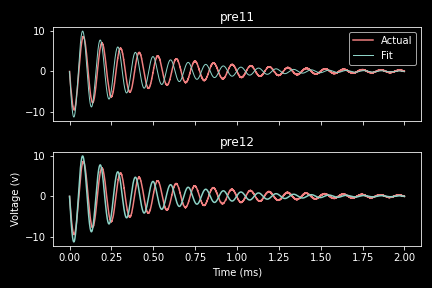
\includegraphics[scale=0.5]{modelofvoltage.png}
  \caption[scale=1.5]{The blue lines are represented by \ref{expon} while the pink correspond to the datavalues found in pre11 and pre12.}
  \label{modelfunction}
\end{figure}

\subsection{Low-Point Circuit}
Draw the wiring for the low-point circuit into the image and include the result in your lab report.

The two series circuits of capacitors and inductors are connected each in parallel with a variance capacitor with capacitance $C_k$. The left and the right capacitor are charged differently with varying charges (same sign).
\begin{figure}[h]
  \centering
  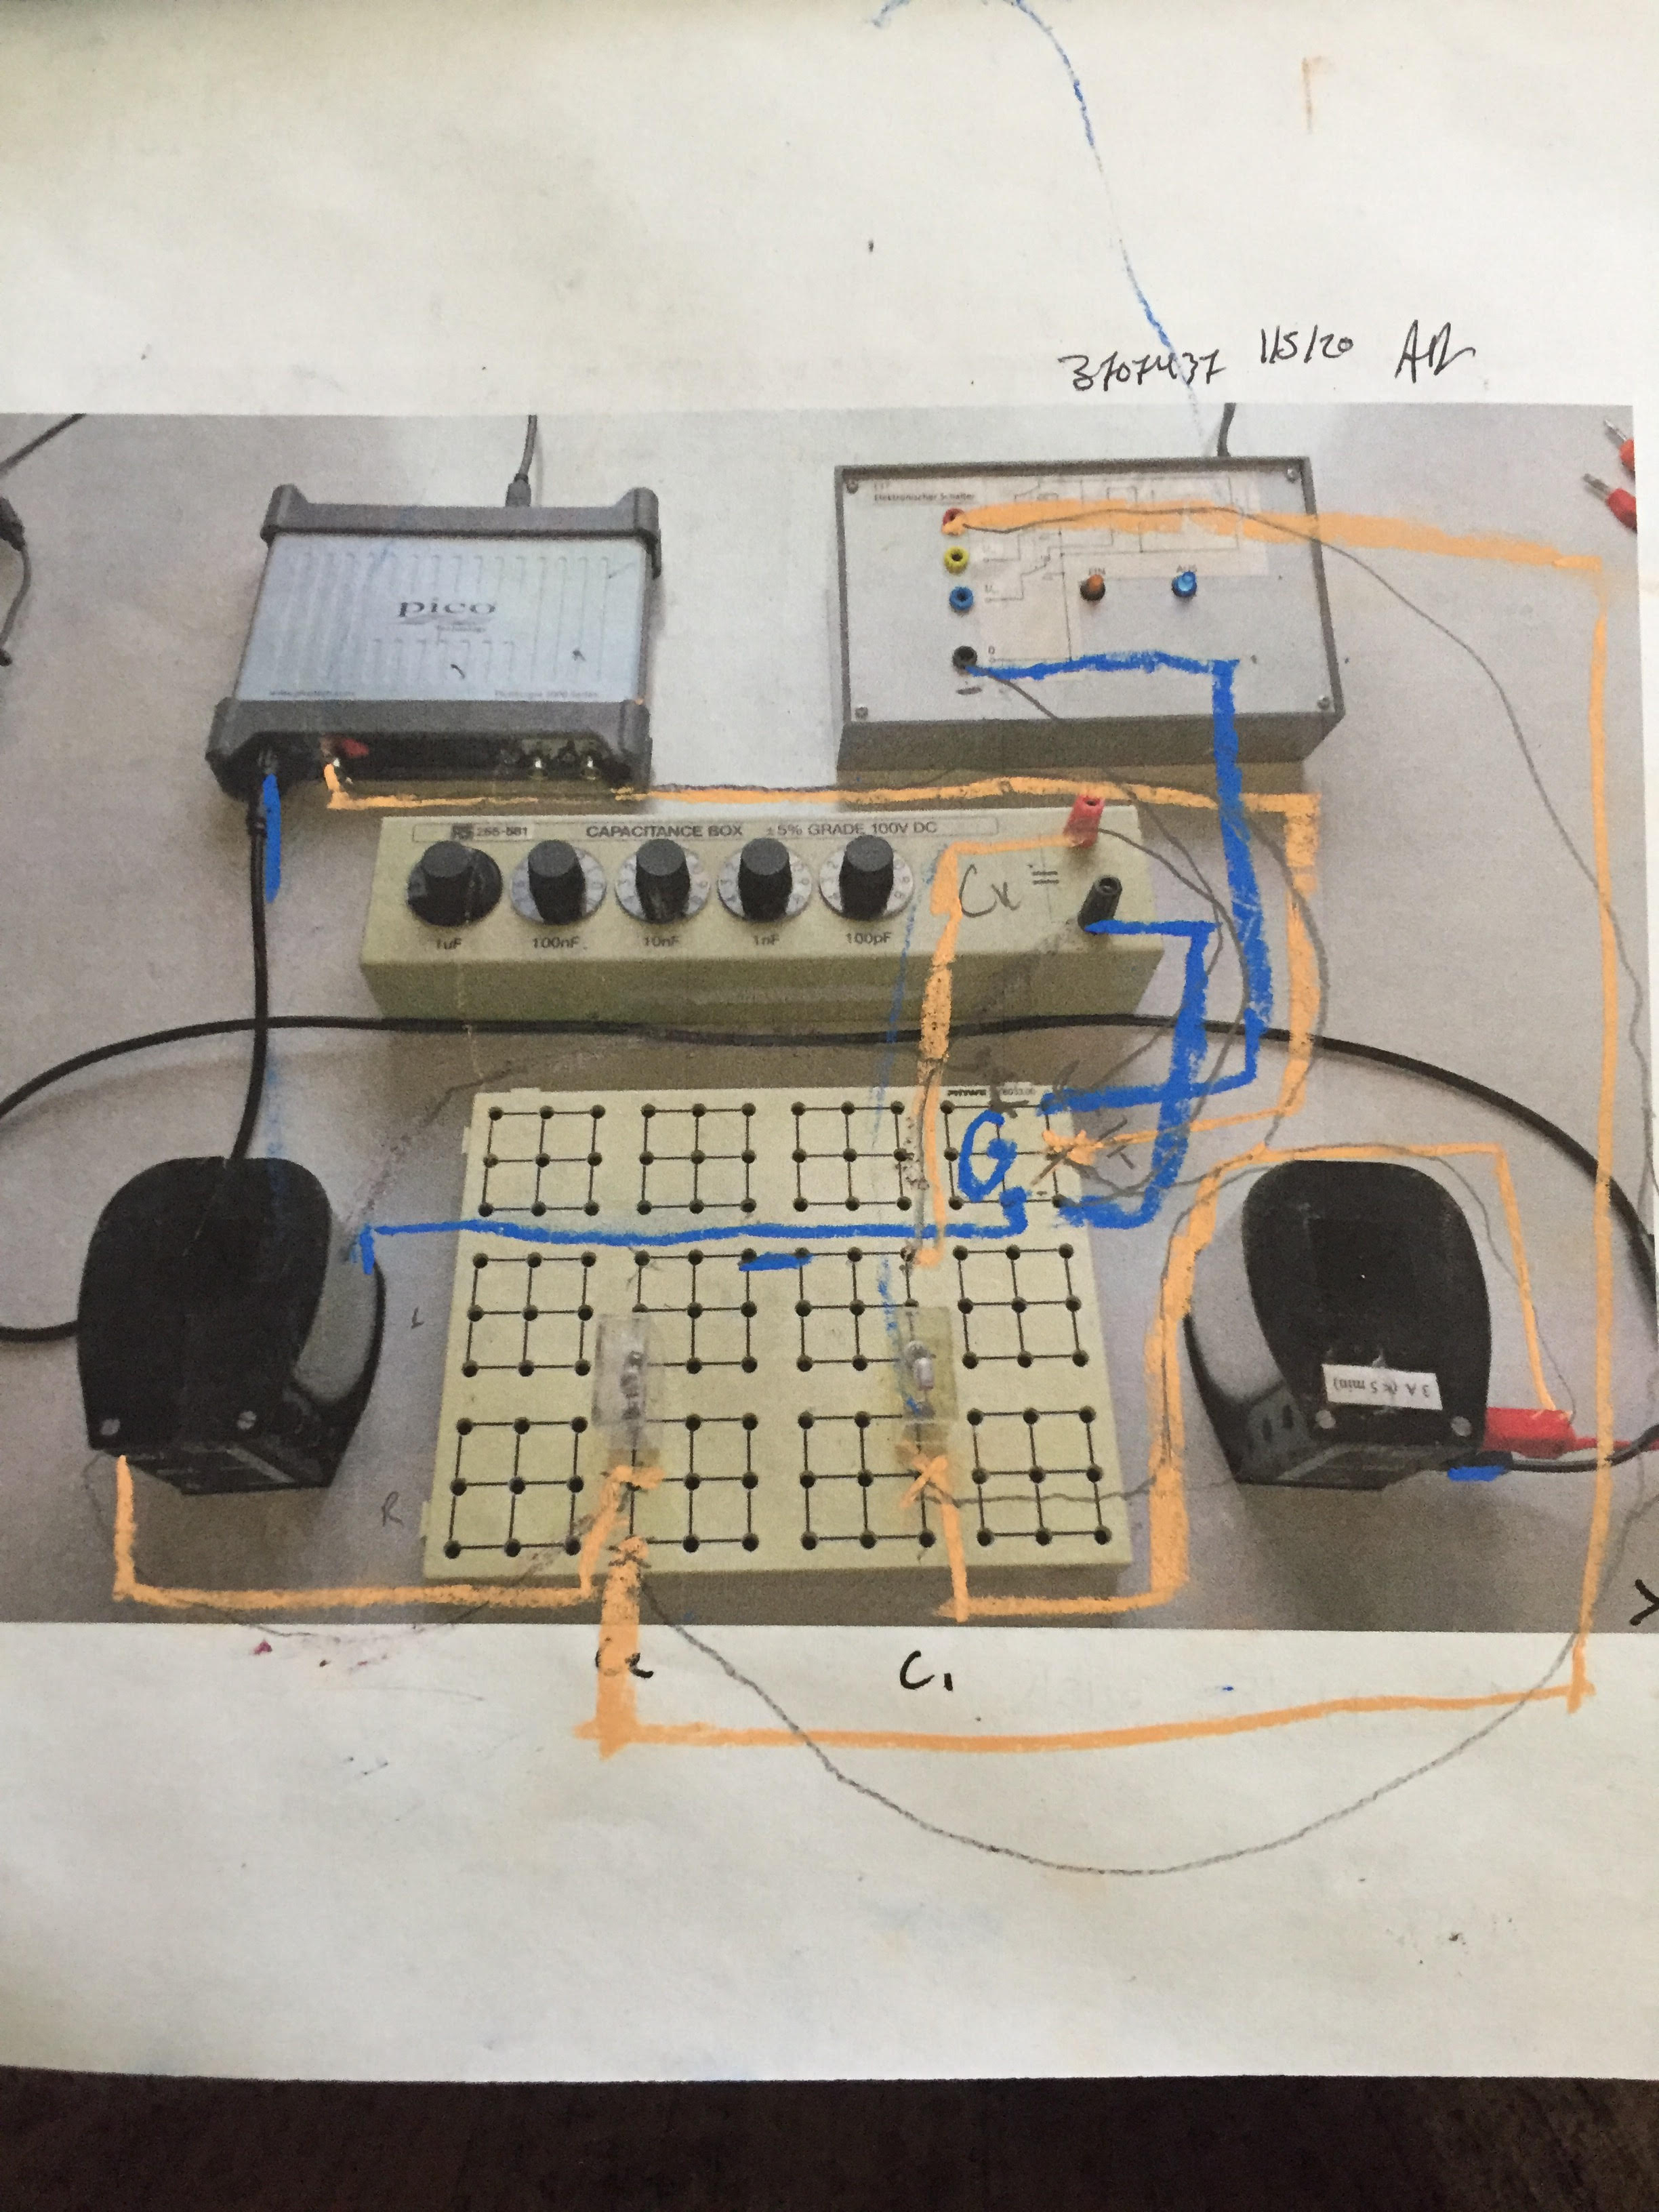
\includegraphics[scale=0.2]{unnamed.jpg}
  \caption{The low point circuit where Blue is - Flow and Orange is +.}
  \label{lowpoint}
\end{figure}
\subsection{High-Point Circuit}
Draw the wiring for the high-point circuit into the image and include the result in your lab report.


\begin{figure}[h]
  \centering
  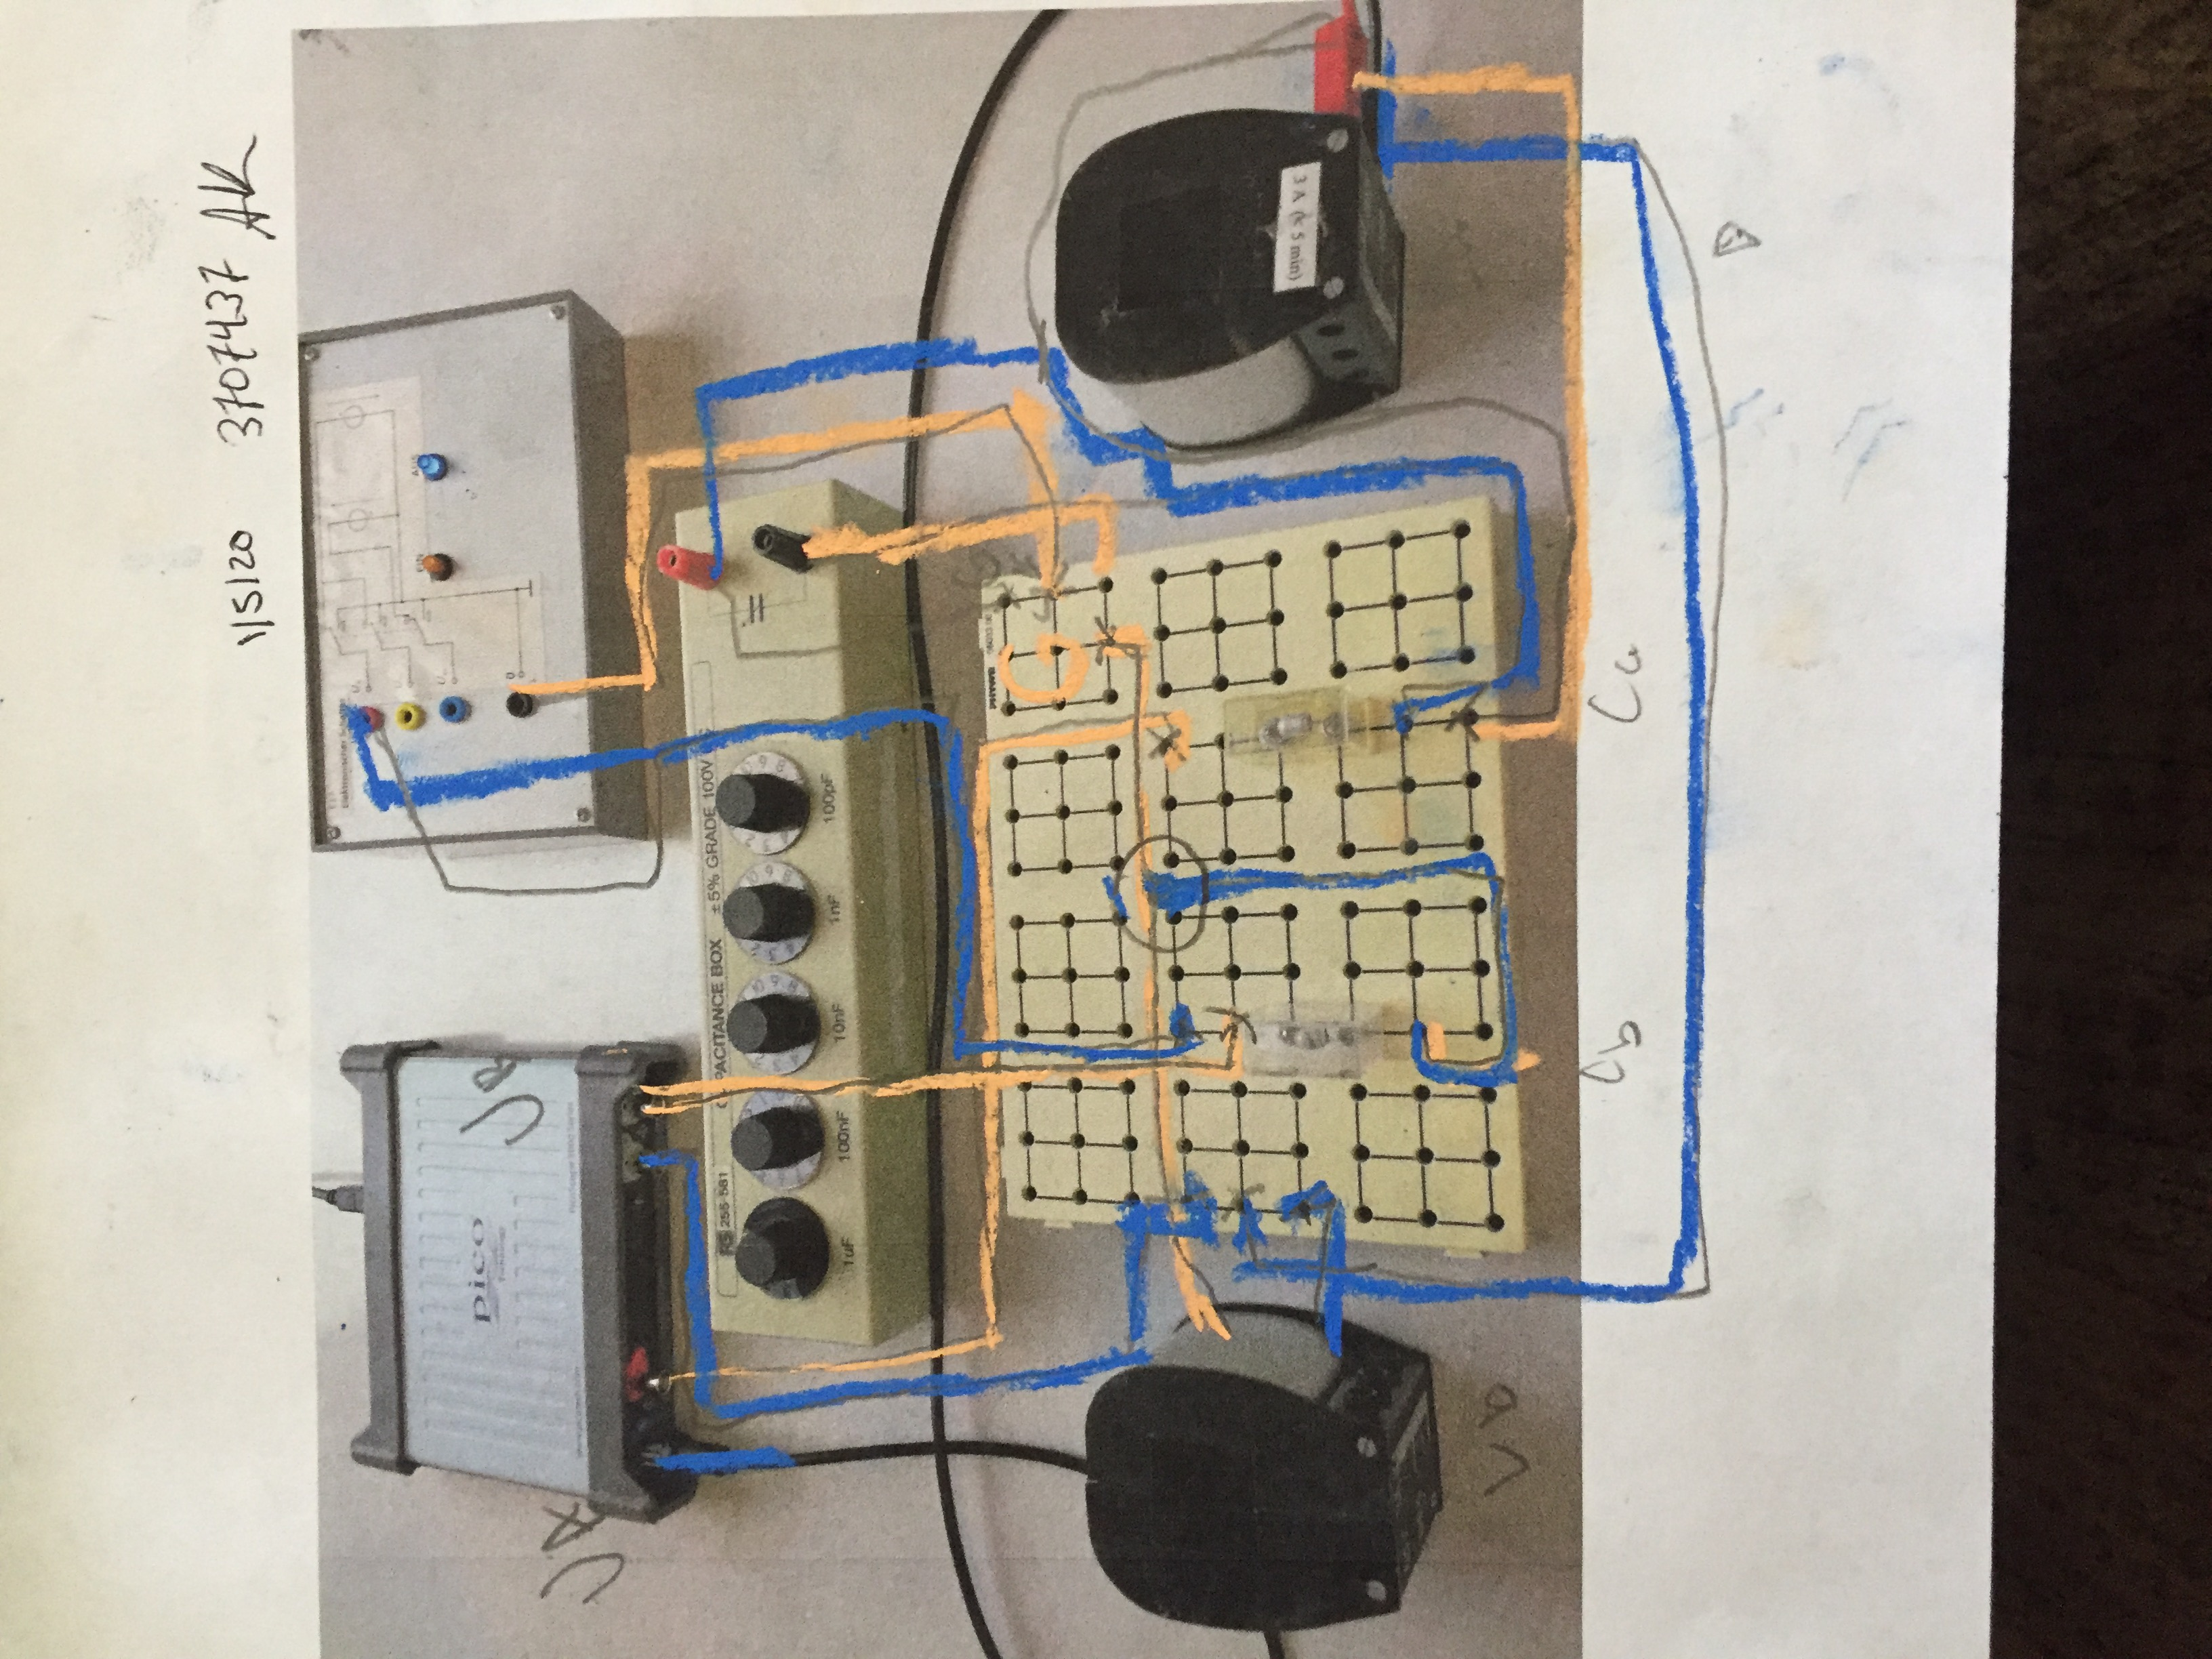
\includegraphics[scale=0.2]{high.jpg}
  \caption{Wiring for High Point Circuit. Blue wire represents + flow while Orange is normally -. The exceptions are for Capacitor B having a blue wire going to ground, and the connection between the Left and Right Inductor.}
  \label{highpoint}
\end{figure}


\section{Task 3: Beat}
Determine the beat period (i) from the time trace and (ii) from the spectrum and compare the two values from dataset Beat1.

Beats appear due to interfence of two sound waves of the same amplitude but slightly different frequencies. The period of the beat is the time interval between two successive maxima or minima, and the number of beats heard per second is the frequency. An awesome example of this is the detection of harmful gasses in mines, where two identical organ pipes are filled with air, one from the mines and the other with clean. Then they are blown together. Should there be a beat from the interference of the two waves, then the mine has bad air \cite{organ_fact}!


\subsection{Beat Period}
The beat period was found by using the two data files given for B0001. From the time series, I calculated the autocorrelation between the initial signal and 5000 other signals, each offset by their corresponding number multiplied by the time step. Please see Figure \ref{beatanal} for example. I found the period to be $1.8869 ms$ through autocorelation. Autocorrelation is outside of the scope of this paper, however I can recommend the following resources to learn more about it: \href{https://www.sciencedirect.com/topics/earth-and-planetary-sciences/autocorrelation}{Articles}. For the frequency we can simply see most common frequency, and use this to calculate the period as $0.7411 ms$. Why such the big difference? Well it may be because the data sample is only one period long. To add more values, one could use autocorrelation to slice the Voltage array and then repeat it, which if it is not included here as a picture, then I point to my github repository, specifically the file \textit{task3.py}.
\begin{figure}[h]
  \centering
  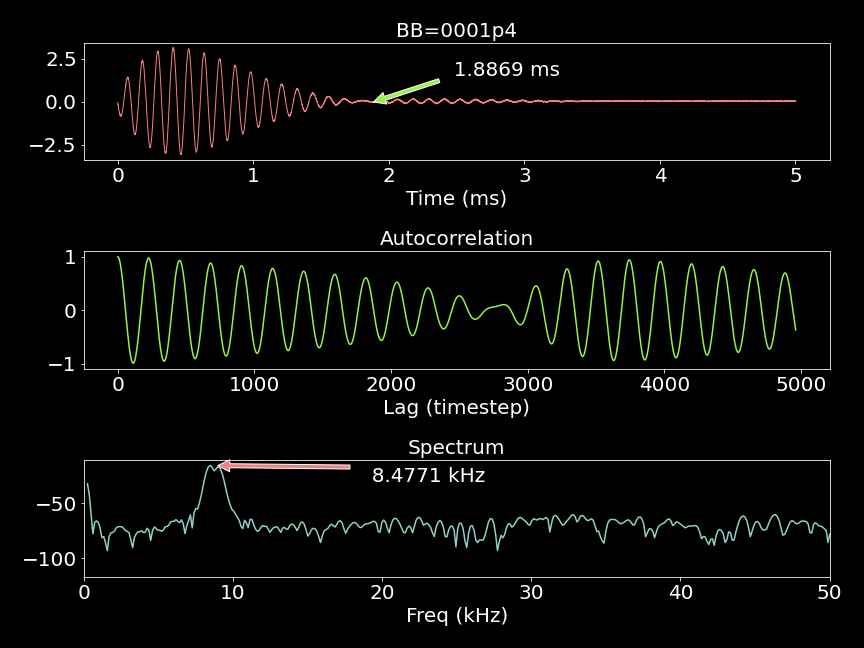
\includegraphics[scale=0.5]{beatanal.png}
  \caption[scale=0.5]{Top: Original Beat, Middle: Autocorrelation between Beat and offset Beat of 5000 timesteps, Bottom: Frequency Spectrum.}
  \label{beatanal}
\end{figure}

\subsection{Mutual Inductance}
We are given a pair of  mutual conductors. Utelizing the curve fit function from scipy, seen in \textit{task4.py} we arrive at \ref{mut}. The math for this can be found in the Lab Instrucutions, and L and C are arbitrary in this case.
\begin{figure}[h]
  \centering
  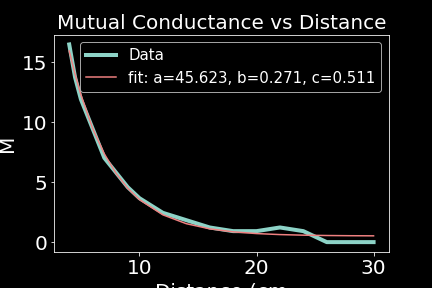
\includegraphics[scale=0.6]{MutualvsDistance.png}
  \caption[scale=0.5]{The inverse power law of Mutual inductance as the inductors get further apart.}
  \label{mut}
\end{figure}

\begin{thebibliography}{9}
\bibitem{latexcompanion}
James W. Cooley and John W. Tukey
\textit{An algorithm for the machine calculation of complex Fourier series}.
Math. Comp. 19 (1965)

\bibitem{FFT-Based}
Cerna, Michael; Harvey, Audrey F.
\textit{The Fundamentals of FFT-Based Signal Analysis and Measurement}
National Instruments Corporation (2000)


\bibitem{organ_fact}
Unknown
\textit{Chemical Analysis of Musical Tones}.
Popular Science, Literary Digest (1899)

\end{thebibliography}

\end{document}
